\chapter{Procesory graficzne}
	\section{Rozwój technologii GPU}
Po raz pierwszy termin ,,procesor graficzny'' użyty został przez firmę NVIDIA w 31 sierpnia 1999 roku. W tym czasie firma wprowadziła na rynek karty graficzne z serii GeForce 256. Układy graficzne, które posiadały procesory wspierające akcelerację 3D istniały już wiele lat wcześniej. Pierwsza na świecie karta graficzna oddana została do użytku w 1981 roku\cite{web-info-komputery}. Była ona częścią komputera o nazwie IBM 5150 i nosiła nazwę MDA (\emph{Monochrome Display Adapter}). Pozwalała na wyświetlenie 25 wierszy po 80 znaków. Początkowa wersja nie dawała możliwości wyświetlania grafiki. Twórcy uważali, że ich komputery wykorzystywane będą wyłącznie w biurach. Okazało się, że popyt na te maszyny istniał wśród odbiorców indywidualnych, którzy zainteresowani byli wykorzystaniem komputerów w celach rozrywkowych. Firma szybko naprawiła swój błąd i wprowadziła na rynek kartę CGA (\emph{Color Graphics Adapter}).

\begin{figure}
\centering
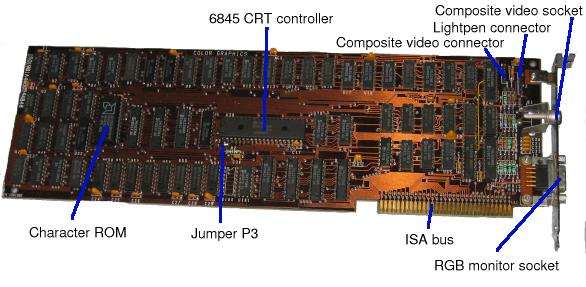
\includegraphics[width=0.5\textwidth]{img/cga.jpg}
\caption{CGA - protoplasta kart graficznych}
\label{fig-cga}
\end{figure}

Karta CGA \ref{fig-cga} wyposażona była w 16KB pamięci przeznaczonej na bufor ramki, który służy do reprezentacji aktualnie wyświetlanego obrazu. Udostępniała dwa tryby tekstowe, co ciekawe, niezgodne z MDA, oraz dwa tryby graficzne. Pierwszy tryb graficzny umożliwiał wyświetlanie 320x200 pikseli z wykorzystaniem 16 kolorów.
Kolejny tryb o wysokiej rozdzielczości 640x200 pikseli umożliwiał wykorzystanie tylko barwy czarnej i białej.

Przez kolejne lata w dziedzinie układów graficznych nie działo się nic przełomowego. Regularnie zwiększano rozdzielczość oraz liczbę obsługiwanych kolorów. Wiązało się to z jednoczesnym wzrostem pojemności dedykowanej pamięci RAM. Sytuacja zmieniła się wraz z powstaniem pierwszych akceleratorów grafiki trójwymiarowej. Jednym z pierwszych akceleratorów był VooDoo. 
	
	
	\section{Standardowy potok graficzny}
	\section{GPGPU}
		\subsection{Pierwsze próby}
		\subsection{OpenCL}
		\subsection{CUDA API}
	\section{Architektura CUDA}